% =========================================================
\subsubsection{Properties of Metrics}
\label{sec:properties-of-metrics}
% =========================================================

% ---- Toolkit ----
\begin{tcolorbox}[colback=gray!6, colframe=gray!40, arc=2pt,
  left=6pt, right=6pt, top=4pt, bottom=4pt,
  title={\small\textbf{Properties of Metrics --- Quick Reference}},
  fonttitle=\small\bfseries]
\small
\begin{tabular}{l l l l}
\toprule
\textbf{Label} & \textbf{Statement} & \textbf{Proof method} & \textbf{Detail} \\
\midrule
D\ref{def:metric}
  & Four axioms: non-neg., identity, symmetry, triangle ineq.
  & Definition
  & \hyperref[def:metric]{$\downarrow$} \\
P\ref{prop:distance-to-itself}
  & $d(x,x) = 0$
  & Axioms 1 + 2
  & \hyperref[prop:distance-to-itself]{$\downarrow$} \\
P\ref{prop:positivity}
  & $x \neq y \Rightarrow d(x,y) > 0$
  & Axioms 1 + 2
  & \hyperref[prop:positivity]{$\downarrow$} \\
P\ref{prop:reverse-triangle}
  & $|d(x,z) - d(y,z)| \le d(x,y)$
  & Triangle ineq.\ + symmetry
  & \hyperref[prop:reverse-triangle]{$\downarrow$} \\
P\ref{prop:generalised-triangle}
  & $d(x_0,x_n) \le \sum_{k=0}^{n-1} d(x_k,x_{k+1})$
  & Induction on $n$
  & \hyperref[prop:generalised-triangle]{$\downarrow$} \\
P\ref{prop:continuity-of-distance}
  & $x \mapsto d(x,z)$ is continuous
  & Reverse triangle ineq.
  & \hyperref[prop:continuity-of-distance]{$\downarrow$} \\
D\ref{def:equivalent-metrics}
  & $d_1 \sim d_2$ iff same open sets
  & Definition
  & \hyperref[def:equivalent-metrics]{$\downarrow$} \\
D\ref{def:ultrametric}
  & $d(x,z) \le \max\{d(x,y),d(y,z)\}$
  & Definition
  & \hyperref[def:ultrametric]{$\downarrow$} \\
T\ref{thm:antimetric-degeneracy}
  & Reversed triangle ineq.\ forces $d \equiv 0$
  & Setting $z=x$
  & \hyperref[thm:antimetric-degeneracy]{$\downarrow$} \\
\bottomrule
\end{tabular}
\end{tcolorbox}

% ---- Metric ----
\begin{tcolorbox}[colback=propbox, colframe=propborder, arc=2pt,
  left=6pt, right=6pt, top=4pt, bottom=4pt,
  title={\small\textbf{Definition (Metric)}},
  fonttitle=\small\bfseries]
\begin{definition}[Metric]
\label{def:metric}
Let $X$ be a set. A function $d : X \times X \to \mathbb{R}$
is called a \emph{metric} on $X$ if for all $x,y,z \in X$:
\begin{enumerate}[label=(M\arabic*)]
  \item\label{M1} $d(x,y) \ge 0$ \hfill (non-negativity)
  \item\label{M2} $d(x,y) = 0 \iff x = y$ \hfill (identity of indiscernibles)
  \item\label{M3} $d(x,y) = d(y,x)$ \hfill (symmetry)
  \item\label{M4} $d(x,z) \le d(x,y) + d(y,z)$ \hfill (triangle inequality)
\end{enumerate}
The pair $(X,d)$ is called a \emph{metric space}.
\end{definition}
\end{tcolorbox}

\begin{remark*}[Fully quantified form]
\[
\forall x,y,z \in X:\quad
d(x,y) \ge 0,\quad
d(x,y)=0 \!\iff\! x=y,\quad
d(x,y)=d(y,x),\quad
d(x,z) \le d(x,y)+d(y,z).
\]
\end{remark*}

\begin{remark*}[Immediate consequences of the axioms]
Three facts follow directly from~\ref{M1} and~\ref{M2} alone,
without any proof beyond unpacking the definitions:
\begin{itemize}
  \item $d(x,x) = 0$ for all $x$ \quad (substitute $y = x$ in~\ref{M2}).
  \item If $d(x,y) = 0$ then $x = y$ \quad (the $(\Leftarrow)$ direction of~\ref{M2}).
  \item If $x \neq y$ then $d(x,y) > 0$ \quad (combine~\ref{M1} with~\ref{M2}).
\end{itemize}
These are listed separately below as labelled propositions so they can be
cited in proofs, but none requires a non-trivial argument.
\end{remark*}

\begin{remark*}[Topology induced by a metric]
The metric $d$ induces a topology on $X$ via open balls
(Definition~\ref{def:open-ball}): a set $U \subseteq X$ is declared open
if every point of $U$ has an open ball centred at it lying inside $U$.
All metric-space analysis --- convergence, continuity, compactness ---
is ultimately grounded in this topology.
\end{remark*}

% ---- Immediate consequences ----

\begin{proposition}[\texorpdfstring{%
  \hyperref[prf:distance-to-itself]{Distance to Itself}%
}{Distance to Itself}]
\label{prop:distance-to-itself}
For all $x \in X$,\quad $d(x,x) = 0$.
\end{proposition}

\begin{proposition}[\texorpdfstring{%
  \hyperref[prf:positivity]{Positivity}%
}{Positivity}]
\label{prop:positivity}
For all $x,y \in X$,\quad $x \neq y \Rightarrow d(x,y) > 0$.
\end{proposition}

% ---- Derived inequalities ----
\begin{tikzpicture}[
  dot/.style={circle,fill,inner sep=1.8pt},
  lbl/.style={font=\small},
  sublbl/.style={font=\scriptsize,text=gray!55!black}
]
\coordinate (x) at (0,0);
\coordinate (y) at (2.8,1.8);
\coordinate (z) at (4.4,0);

% Broken path x->y->z (blue, thicker)
\draw[blue!70!black, line width=1.6pt] (x) -- (y) -- (z);

% Direct path x->z (red)
\draw[red!70!black, line width=1.4pt, dashed] (x) -- (z);

% Points
\node[dot] at (x) {};  \node[dot] at (y) {};  \node[dot] at (z) {};
\node[lbl,anchor=north east] at ($(x)+(-0.05,-0.1)$) {$x$};
\node[lbl,anchor=south]      at ($(y)+(0,0.12)$)     {$y$};
\node[lbl,anchor=north west] at ($(z)+(0.05,-0.1)$)  {$z$};

% d(x,y) label along x->y
\node[sublbl,anchor=south east,rotate=33]
  at ($(x)!0.5!(y)+(-0.12,0.1)$) {$d(x,y)$};

% d(y,z) label along y->z
\node[sublbl,anchor=south west,rotate=-27]
  at ($(y)!0.5!(z)+(0.1,0.1)$) {$d(y,z)$};

% d(x,z) label below direct path
\node[sublbl,text=red!70!black,anchor=north]
  at ($(x)!0.5!(z)+(0,-0.18)$) {$d(x,z)$};

% Inequality annotation
\node[lbl,align=center] at ($(x)!0.5!(z)+(0,-1.0)$)
  {$d(x,z) \;\le\; d(x,y) + d(y,z)$\\[3pt]
   {\scriptsize\color{gray!60!black}direct path $\le$ broken path}};

% Legend
\draw[blue!70!black,line width=1.4pt] (3.2,2.4) -- (4.1,2.4);
\node[sublbl,anchor=west] at (4.15,2.4) {broken path};
\draw[red!70!black,line width=1.2pt,dashed] (3.2,2.0) -- (4.1,2.0);
\node[sublbl,text=red!70!black,anchor=west] at (4.15,2.0) {direct path};
\end{tikzpicture}
\begin{proposition}[\texorpdfstring{%
  \hyperref[prf:reverse-triangle]{Reverse Triangle Inequality}%
}{Reverse Triangle Inequality}]
\label{prop:reverse-triangle}
For all $x,y,z \in X$,
\[
|d(x,z) - d(y,z)| \le d(x,y).
\]
\end{proposition}
\begin{tikzpicture}[
  dot/.style={circle,fill,inner sep=1.8pt},
  lbl/.style={font=\small},
  sublbl/.style={font=\scriptsize,text=gray!55!black}
]
\coordinate (x) at (0,0);
\coordinate (y) at (1.6,0);
\coordinate (z) at (4.8,0);

% Fixed point z shown above; draw connecting lines
\coordinate (zfixed) at (3.2,2.8);

% Lines x->zfixed and y->zfixed
\draw[blue!65!black, line width=1.2pt] (x) -- (zfixed);
\draw[orange!75!black, line width=1.2pt] (y) -- (zfixed);

% d(x,y) line
\draw[gray!60, line width=1.0pt, <->] ($(x)+(0,-0.45)$) -- ($(y)+(0,-0.45)$);
\node[sublbl,anchor=north] at ($(x)!0.5!(y)+(0,-0.5)$) {$d(x,y)$};

% d(x,z) label
\node[sublbl,text=blue!65!black,anchor=east,rotate=60]
  at ($(x)!0.5!(zfixed)+(-0.18,0)$) {$d(x,z)$};

% d(y,z) label
\node[sublbl,text=orange!75!black,anchor=west,rotate=-48]
  at ($(y)!0.5!(zfixed)+(0.15,0)$) {$d(y,z)$};

% Points
\node[dot] at (x) {};
\node[dot] at (y) {};
\node[dot,fill=gray!60] at (zfixed) {};

\node[lbl,anchor=north] at ($(x)+(0,-0.08)$) {$x$};
\node[lbl,anchor=north] at ($(y)+(0,-0.08)$) {$y$};
\node[lbl,anchor=south,text=gray!60] at ($(zfixed)+(0,0.1)$) {$z$ (fixed)};

% Annotation
\node[lbl,align=center] at (2.4,-1.2)
  {$|d(x,z) - d(y,z)| \;\le\; d(x,y)$\\[3pt]
   {\scriptsize\color{gray!60!black}moving from $x$ to $y$ changes distance to $z$ by at most $d(x,y)$}};
\end{tikzpicture}


\begin{remark*}[Intuition]
The reverse triangle inequality says that the difference in distances
from two points to a fixed reference cannot exceed the distance between
the two points themselves.
It is the key tool for proving that $x \mapsto d(x,z)$ is continuous.
\end{remark*}

\begin{proposition}[\texorpdfstring{%
  \hyperref[prf:generalised-triangle]{Generalised Triangle Inequality}%
}{Generalised Triangle Inequality}]
\label{prop:generalised-triangle}
For $x_0, x_1, \dots, x_n \in X$,
\[
d(x_0, x_n) \le \sum_{k=0}^{n-1} d(x_k, x_{k+1}).
\]
\end{proposition}

\begin{remark*}[Intuition]
The total length of any polygonal path from $x_0$ to $x_n$
is at least the direct distance.
The proof is a straightforward induction applying~\ref{M4} at each step.
\end{remark*}

% ---- Continuity of distance ----

\begin{proposition}[\texorpdfstring{%
  \hyperref[prf:continuity-of-distance]{Continuity of Distance}%
}{Continuity of Distance}]
\label{prop:continuity-of-distance}
For fixed $z \in X$, the function $f : X \to \mathbb{R}$ defined by
$f(x) := d(x,z)$ is continuous.
\end{proposition}

\begin{remark*}[Consequence]
This means convergence $x_n \to x$ in $(X,d)$ implies
$d(x_n,z) \to d(x,z)$ for every fixed $z$.
In other words, the metric function itself is continuous as a map
from $(X,d)$ to $(\mathbb{R}, |\cdot|)$.
\end{remark*}

% ---- Equivalent metrics ----
\begin{tcolorbox}[colback=propbox, colframe=propborder, arc=2pt,
  left=6pt, right=6pt, top=4pt, bottom=4pt,
  title={\small\textbf{Definition (Equivalent Metrics)}},
  fonttitle=\small\bfseries]
\begin{definition}[Equivalent Metrics]
\label{def:equivalent-metrics}
Let $d_1$ and $d_2$ be two metrics on the same set $X$.
They are called \emph{equivalent} (written $d_1 \sim d_2$) if they induce
the same topology, i.e.\ if every open set in $(X,d_1)$ is open in
$(X,d_2)$ and vice versa.

A sufficient condition is the existence of constants $c, C > 0$ such that
\[
c\, d_1(x,y) \;\le\; d_2(x,y) \;\le\; C\, d_1(x,y)
\quad \forall x,y \in X.
\]
When this holds, $d_1$ and $d_2$ are called \emph{strongly equivalent}.
\end{definition}
\end{tcolorbox}

\begin{remark*}[Fully quantified form]
\[
d_1 \sim d_2
\iff
\forall U \subseteq X,\;
\bigl(U \in \tau_{d_1} \iff U \in \tau_{d_2}\bigr),
\]
where $\tau_d$ denotes the topology induced by $d$.
\end{remark*}

\begin{remark*}[Consequence]
Equivalent metrics agree on all topological properties: convergence,
continuity, open and closed sets, compactness, connectedness.
They may disagree on metric properties such as completeness and uniform
continuity, which depend on the specific distances, not just the topology.
On $\mathbb{R}^n$, all norms induce strongly equivalent metrics.
\end{remark*}

% ---- Ultrametric ----
\begin{tcolorbox}[colback=propbox, colframe=propborder, arc=2pt,
  left=6pt, right=6pt, top=4pt, bottom=4pt,
  title={\small\textbf{Definition (Ultrametric)}},
  fonttitle=\small\bfseries]
\begin{definition}[Ultrametric]
\label{def:ultrametric}
Let $(X,d)$ be a metric space.
The metric $d$ is called an \emph{ultrametric} if for all $x,y,z \in X$,
\[
d(x,z) \le \max\{\, d(x,y),\, d(y,z) \,\}.
\]
\end{definition}
\end{tcolorbox}

\begin{remark*}[Relation to the ordinary triangle inequality]
The ultrametric inequality $d(x,z) \le \max\{d(x,y), d(y,z)\}$
implies the ordinary triangle inequality
$d(x,z) \le d(x,y) + d(y,z)$,
since $\max\{a,b\} \le a + b$ for $a,b \ge 0$.
So every ultrametric is a metric, but not every metric is an ultrametric.
\end{remark*}

\begin{remark*}[Intuition]
In an ultrametric space, all triangles are \emph{isosceles}:
if $d(x,y) \neq d(y,z)$, then $d(x,z) = \max\{d(x,y), d(y,z)\}$.
Balls have a striking property: any point inside a ball is a centre of
that ball, and any two balls are either disjoint or one contains the other.
\end{remark*}

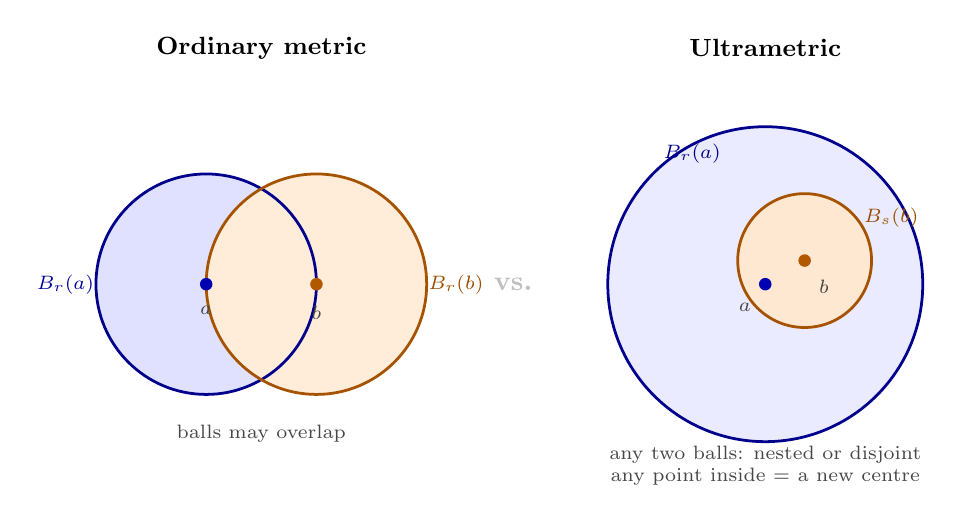
\begin{tikzpicture}[
  dot/.style={circle,fill,inner sep=1.6pt},
  lbl/.style={font=\small},
  sublbl/.style={font=\scriptsize,text=gray!55!black}
]

% ---- LEFT: Ordinary metric — balls can overlap ----
\begin{scope}[shift={(-3.2,0)}]
  \node[lbl,font=\small\bfseries] at (0,3.0) {Ordinary metric};

  % Two overlapping balls
  \fill[blue!12] (-0.7,0) circle (1.4cm);
  \fill[orange!15] (0.7,0) circle (1.4cm);
  \draw[blue!55!black, line width=1.0pt] (-0.7,0) circle (1.4cm);
  \draw[orange!65!black, line width=1.0pt] (0.7,0) circle (1.4cm);

  \node[dot,fill=blue!70!black] at (-0.7,0) {};
  \node[dot,fill=orange!70!black] at (0.7,0) {};
  \node[sublbl,anchor=north] at (-0.7,-0.15) {$a$};
  \node[sublbl,anchor=north] at (0.7,-0.15)  {$b$};
  \node[sublbl,text=blue!60!black,anchor=east] at (-2.0,0) {$B_r(a)$};
  \node[sublbl,text=orange!60!black,anchor=west] at (2.0,0) {$B_r(b)$};

  % Overlap label
  \node[sublbl,align=center] at (0,-1.9) {balls may overlap};
\end{scope}

% ---- RIGHT: Ultrametric — balls are nested or disjoint ----
\begin{scope}[shift={(3.2,0)}]
  \node[lbl,font=\small\bfseries] at (0,3.0) {Ultrametric};

  % Outer ball
  \fill[blue!8] (0,0) circle (2.0cm);
  \draw[blue!55!black, line width=1.0pt] (0,0) circle (2.0cm);

  % Inner ball (nested inside outer)
  \fill[orange!18] (0.5,0.3) circle (0.85cm);
  \draw[orange!65!black, line width=1.0pt] (0.5,0.3) circle (0.85cm);

  \node[dot,fill=blue!70!black] at (0,0) {};
  \node[dot,fill=orange!70!black] at (0.5,0.3) {};
  \node[sublbl,anchor=north east] at (-0.06,-0.12) {$a$};
  \node[sublbl,anchor=north west] at (0.56,0.18) {$b$};
  \node[sublbl,text=blue!55!black,anchor=south west] at ({-2.0*0.707},{2.0*0.707}) {$B_r(a)$};
  \node[sublbl,text=orange!60!black] at (1.6,0.85) {$B_s(b)$};

  % Key property annotation
  \node[sublbl,align=center] at (0,-2.3)
    {any two balls: nested or disjoint\\
     any point inside = a new centre};
\end{scope}

% Divider label
\node[lbl,text=gray!50,font=\normalsize\bfseries] at (0,0) {vs.};

\end{tikzpicture}



\begin{example*}[Discrete metric is an ultrametric]
The discrete metric
\[
d_{\mathrm{disc}}(x,y) :=
\begin{cases} 0 & x = y, \\ 1 & x \neq y \end{cases}
\]
is an ultrametric: if $x \neq z$ then at least one of $d(x,y), d(y,z)$
equals $1$, so $\max\{d(x,y), d(y,z)\} = 1 = d(x,z)$.
\end{example*}

\begin{example*}[$p$-adic metric]
For a prime $p$, the $p$-adic metric on $\mathbb{Q}$ is defined by
$d_p(x,y) := p^{-v_p(x-y)}$ where $v_p(n)$ is the largest power of $p$
dividing $n$.
This is the canonical non-trivial ultrametric and is the foundation of
$p$-adic analysis.
\end{example*}

% ---- Antimetric ----
\begin{tcolorbox}[colback=propbox, colframe=propborder, arc=2pt,
  left=6pt, right=6pt, top=4pt, bottom=4pt,
  title={\small\textbf{Definition (Antimetric)}},
  fonttitle=\small\bfseries]
\begin{definition}[Antimetric]
\label{def:antimetric}
Let $X$ be a set. A function $d : X \times X \to \mathbb{R}$ is called
an \emph{antimetric} if for all $x,y,z \in X$:
\begin{enumerate}[label=(A\arabic*)]
  \item $d(x,y) \ge 0$,
  \item $d(x,y) = 0 \iff x = y$,
  \item $d(x,y) = d(y,x)$,
  \item $d(x,z) \ge d(x,y) + d(y,z)$ \hfill (reversed triangle inequality)
\end{enumerate}
\end{definition}
\end{tcolorbox}

\begin{remark*}[Why antimetrics are pathological]
The reversed triangle inequality forces the opposite of the familiar
geometry: going through an intermediate point can only make distances
\emph{smaller}, never larger.
As a consequence, antimetric spaces admit no meaningful notion of
convergence, continuity, or compactness.
The triangle inequality is not a technical convenience --- it is the
structural axiom that makes analysis possible.
The theorem below shows the damage is total: the reversed inequality
collapses every antimetric to the zero function.
\end{remark*}

% ---- Degeneracy theorem ----
\begin{tcolorbox}[colback=thmbox, colframe=thmborder, arc=2pt,
  left=6pt, right=6pt, top=4pt, bottom=4pt,
  title={\small\textbf{Theorem (Degeneracy of the Antimetric)}},
  fonttitle=\small\bfseries]
\begin{theorem}[\texorpdfstring{%
  \hyperref[prf:antimetric-degeneracy]{Degeneracy of the Antimetric}%
}{Degeneracy of the Antimetric}]
\label{thm:antimetric-degeneracy}
Let $X$ be a set and let $d : X \times X \to [0,\infty)$ satisfy the
reversed triangle inequality:
\[
d(x,z) \ge d(x,y) + d(y,z)
\quad \forall\, x,y,z \in X.
\]
Then $d(x,y) = 0$ for all $x,y \in X$.
In particular, if the separation axiom $d(x,y) = 0 \Rightarrow x = y$
also holds, then $|X| \le 1$.
\end{theorem}
\end{tcolorbox}

\begin{remark*}[Fully quantified form]
\[
\bigl(\forall x,y,z \in X,\; d(x,z) \ge d(x,y)+d(y,z)\bigr)
\;\Rightarrow\;
\bigl(\forall x,y \in X,\; d(x,y) = 0\bigr).
\]
\end{remark*}

\begin{remark*}[Proof shape]
Set $z = x$ in the reversed inequality to get
$d(x,x) \ge d(x,y) + d(y,x) = 2\,d(x,y)$.
Since $d(x,x) = 0$ by non-negativity and identity, this gives
$0 \ge 2\,d(x,y)$, hence $d(x,y) \le 0$.
Non-negativity then forces $d(x,y) = 0$.
\end{remark*}